\documentclass[11pt]{article}
\usepackage{graphicx}
\usepackage{amsmath}
\usepackage{hyperref}

\title{EnterpriseSynth: A Schema-Aware Agentic Framework for Generating Verified SFT and Evaluation Datasets from OpenAPI Specifications}
\author{Rashmi Thimmaraju}
\date{}

\begin{document}
\maketitle

\begin{abstract}
Enterprise adoption of autonomous Large Language Model (LLM) agents is severely bottlenecked by
the data cold-start problem. Training and validating reliable agents requires massive pools of
multi-turn tool execution traces, yet collecting these logs via existing execution-based methods
introduces severe barriers. Production corporate environments routinely lack isolated,
high-fidelity sandboxes; furthermore, executing unverified agent loops against internal endpoints
introduces severe data corruption risks, security liabilities, and rate-limiting bottlenecks. We
present \textbf{EnterpriseSynth}, a zero-execution framework that ingests abstract OpenAPI/Swagger
specifications to synthesize verified Supervised Fine-Tuning (SFT) interaction traces and complex
evaluation records entirely offline. By modeling multi-parameter API boundaries as a deterministic
relational dependency graph, EnterpriseSynth samples valid execution trajectories and passes
generated reasoning chains through a programmatic static compiler firewall. Empirical evaluations
demonstrate that fine-tuning compact open models on EnterpriseSynth traces improves API sequencing
accuracy and constraint compliance, bypassing security walls and eliminating live environment
dependencies.
\end{abstract}

\section{Introduction}
The paradigm of software engineering and workflow automation is experiencing a structural shift
toward autonomous, tool-augmented Large Language Model (LLM) agents. By translating
non-deterministic natural language intents into deterministic sequences of external system
transactions---modeled as structured web interfaces via OpenAPI or Swagger specifications---agents
possess the theoretical capacity to orchestrate highly complex enterprise operations.

\begin{figure}[t]
\centering
% TODO: replace with local system vector graphic mapping graph parsing logic
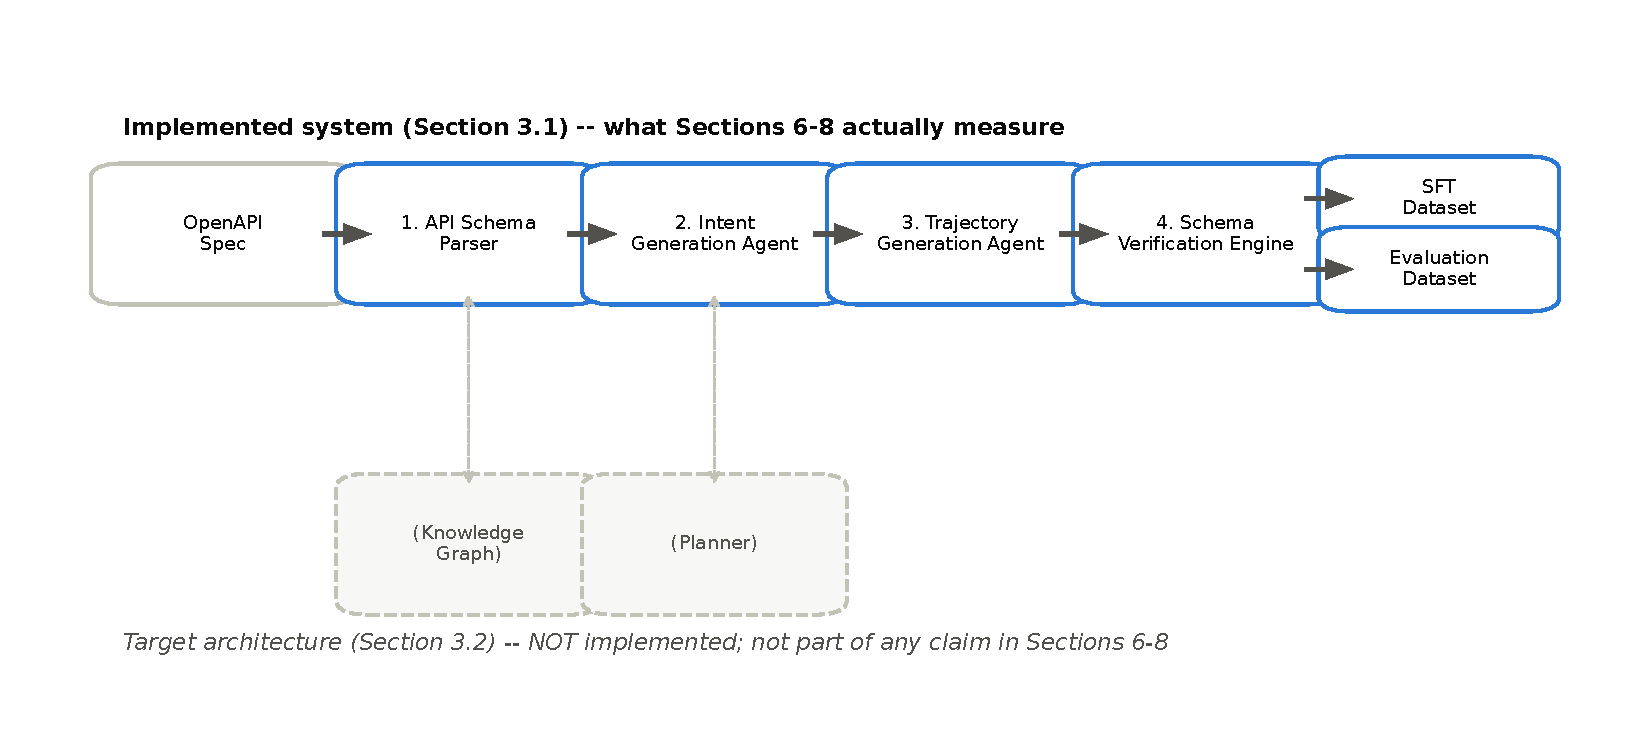
\includegraphics[width=\columnwidth]{enterprisesynth_pipeline_diagram.pdf}
\caption{The EnterpriseSynth Zero-Execution Architectural Matrix vs Traditional Live Pipelines.}
\label{fig:pipeline_matrix}
\end{figure}

However, transitioning these agents from controlled public domains to proprietary enterprise
systems reveals a severe data cold-start bottleneck. Out-of-the-box foundation models exhibit poor
zero-shot performance on enterprise tool configurations; they frequently violate JSON payload
definitions, hallucinate non-existent parameter fields, and fail to track cascading variables
across multi-step execution paths. Mitigating these structural failures necessitates robust
Supervised Fine-Tuning (SFT) alongside highly localized evaluation tracks.

To populate these training datasets, state-of-the-art synthetic data generation engines rely
exclusively on an active execution paradigm. Frameworks such as ToolBench~\cite{qin2023toolbench}
connect target foundation models to live execution servers or populated network backends,
recording real-world system responses to construct functional interaction traces. While viable
for public web extensions, this operational assumption collapses behind the enterprise firewall
due to a three-fold conflict we term the \textit{Execution Paradox}:
\begin{enumerate}
    \item \textbf{Sandbox Absences:} High-fidelity staging copies populated with realistic data
    states rarely exist for specialized, internal corporate software clusters.
    \item \textbf{Data Privacy and State Vulnerability:} Running autonomous exploratory agent loops
    against production layers introduces catastrophic risks, including the corruption of
    operational state variables, violation of security compliance boundaries, and unintended
    execution of destructive actions.
    \item \textbf{Throughput Constraints:} Active generation over network layers is inherently
    bounded by high request latencies and rigid infrastructure rate-limiting rules.
\end{enumerate}

To resolve this paradox, we present \textbf{EnterpriseSynth}, a zero-execution synthesis matrix
that completely decouples agent data generation from system execution. EnterpriseSynth shifts the
data-gathering pipeline from a runtime extraction challenge to a static compiler optimization
problem. Given an abstract enterprise API schema definition, our framework programmatically maps
endpoints into a directed relational parameter graph, samples valid multi-step operational
trajectories, utilizes an offline inference driver to synthesize textual reasoning paths, and
strictly enforces data typing boundaries through an automated static constraint validation
firewall.

The closest existing architecture to this offline synthesis approach is
AgentInstruct~\cite{mitra2024agentinstruct}, whose agentic multi-flow pipeline generates tool-use
training data without executing any tool, simulating responses via the LLM itself. However, when
seeded only from source code, AgentInstruct's content-transformation stage must synthesize an API
description from the code or have the LLM hypothesize additional APIs it believes exist, with no
ground-truth check against a real interface definition; its quality control is a soft
Suggester-Editor refinement loop plus a held-out, post-hoc LLM-judged benchmark, not a per-sample
structural gate. We adapt its agentic-flow architecture to ingest a real target-organization
OpenAPI/Swagger spec directly (removing the hallucination step entirely, since the schema is
already ground truth), replace its post-hoc judging with a hard static constraint validator checked
against the spec, and extend the pipeline to jointly emit intent-spec-tied evaluation records. We
position against the two execution-dependent alternatives in our review, API-Bank~\cite{li2023apibank}
and ToolBench~\cite{qin2023toolbench}, on safety and availability grounds: both ground their
training data in real API calls (API-Bank against reproducibility-constrained real databases,
ToolBench via roughly 470,000 live RapidAPI calls during annotation), which is exactly the
dependency the Execution Paradox rules out for most enterprise API surfaces.

\subsection{Summary of Contributions}
Our core architectural contributions to the research frontier are structured as follows:
\begin{itemize}
    \item We introduce a formal software framework for zero-execution agent data generation that
    ingests production-tier OpenAPI schemas to output multi-turn instruction traces without a
    single live backend connection.
    \item We detail a deterministic relational graph engine that translates structural parameter
    schemas into explicit dependency chains to guide agent sequencing without data
    hallucinations.
    \item We release a programmatic static constraint validator that mimics compiler-level
    firewalls to verify schema parameters, JSON syntax configurations, and variable types
    completely offline.
    \item We demonstrate that models optimized with our synthetic data distribution achieve
    significant improvements in tool-sequencing success rates on our evaluation suite.
    % NOTE: eval-suite name TBD pending the EnterpriseBench naming-collision decision --
    % see DESIGN_DOC.md's open item. Do not finalize "EnterpriseBench" as the name here
    % without resolving that first.
\end{itemize}

\section{Related Work}
Our review covers two lineages: general-purpose synthetic instruction generation, and tool/API
data generation specifically.

\subsection{Synthetic Instruction Generation}
\textbf{Self-Instruct}~\cite{wang2022selfinstruct} bootstraps instruction-tuning data from a
model's own generations: starting from 175 human-written seed tasks, it iteratively prompts the
model for new instructions, routes classification vs.\ non-classification tasks to different
instance-generation strategies (output-first vs.\ input-first, to avoid label bias), and filters
results with ROUGE-L similarity thresholds, keyword blocklists, and format/degeneracy heuristics.
No execution and no tool/API notion is involved anywhere in the method.
\textbf{Evol-Instruct/WizardLM}~\cite{xu2023wizardlm} instead evolves existing instructions along
controlled axes -- in-depth evolving (add constraints, deepen, concretize, increase reasoning
steps, complicate the input format) and in-breadth evolving (generate novel same-domain
instructions) -- with an ``elimination evolving'' step discarding degenerate evolutions. Neither
paper touches tool-use or API grounding at all; both are precedents for cheap, execution-free,
heuristically-filtered synthetic data at scale.

\textbf{AgentInstruct}~\cite{mitra2024agentinstruct} is the closest architectural precedent overall:
an agentic, three-flow pipeline (content transformation, taxonomy-driven seed instruction
generation, and Suggester-Editor iterative refinement) that produced the 25-million-pair dataset
behind Orca-3. Its \texttt{tool\_use} skill category is seeded from either a code snippet or an
API description; critically, when only code is available, a transformation agent
\textit{synthesizes} an API description from it, and a retrieval agent or the LLM itself may
\textit{hypothesize} additional APIs it believes exist in the library, with no ground-truth check.
Tool responses in the resulting traces are LLM-simulated JSON, never executed. Verification is a
soft editorial loop (Suggester-Editor) plus a held-out, GPT-4-judged benchmark (Orca-Bench, 1,700
samples) computed \textit{after} data generation, not a per-sample structural filter -- the authors
themselves note that ``synthetic data may not perfectly replicate the complexity and nuances of
real-world data.''

\subsection{Execution-Dependent Tool-Use Data}
\textbf{API-Bank}~\cite{li2023apibank} evaluates tool proficiency across retrieval, execution, and
planning tiers using real (though reproducibility-constrained -- results are hard-coded from a
fixed query time) database backends. Its 1,888 training dialogues are themselves synthesized by an
automated 5-agent pipeline, at 98\% lower cost than human annotation and a 94\% validity rate --
evidence that agentic pipelines can approximate human-annotation quality even for tool dialogues --
but its 314-dialogue evaluation set is manually annotated, and correctness is judged by comparing
predicted vs.\ gold API calls for behavioral equivalence.
\textbf{ToolLLM/ToolBench}~\cite{qin2023toolbench} scales this further: 16,464 real RapidAPI
endpoints, ChatGPT-generated instructions, and a depth-first search-based decision tree (DFSDT)
solution-path annotator that \textit{actually calls} the sampled real API at each step (roughly
470,000 live calls logged during annotation) to obtain ground-truth responses, scored downstream by
ToolEval's pass-rate/win-rate LLM judge (87\%/80\% agreement with human raters).

Both are effective precisely because they ground responses in real execution -- which is exactly
the capability that collapses behind an enterprise firewall (Section~1's Execution Paradox): no
sandbox for internal systems, security/PII exposure from live calls, and infrastructure rate limits.

\subsection{Research Gap}
Current research demonstrates important advances in tool-using language models and synthetic
instruction generation, yet several limitations remain: ToolLLM/ToolBench focus on public APIs and
require large collections of externally available, callable services; API-Bank evaluates
API-calling agents through executable APIs, making it dependent on live systems; and
Self-Instruct, WizardLM, and AgentInstruct synthesize instruction-following data from text or code
rather than from structured API specifications, leaving AgentInstruct's tool-use flow exposed to
API hallucination when no real spec is available. No existing framework automatically converts an
enterprise OpenAPI specification into both verified SFT trajectories and evaluation records
suitable for training and assessing enterprise LLM agents without live API execution. This gap
motivates EnterpriseSynth, a schema-aware framework that automatically synthesizes user intents,
reasoning traces, API call sequences, expected outputs, and verification metadata directly from
OpenAPI specifications, enabling enterprises to bootstrap both agent training and evaluation from
API documentation alone.

\section{Methodology}
EnterpriseSynth is a seven-stage offline pipeline (Figure~\ref{fig:pipeline_matrix}), each stage
addressing a specific gap identified in Section~2's research-gap analysis.

\textbf{1. API Schema Parser.} Ingests the OpenAPI/Swagger spec and extracts endpoints,
parameters, authentication requirements, and response schemas.

\textbf{2. API Knowledge Graph Builder.} Constructs a directed graph
$\mathcal{G} = (\mathcal{V}, \mathcal{E})$ with endpoints, objects, and parameters as nodes, and
dependency, sequential-workflow, and object-relation edges. Unlike
AgentInstruct~\cite{mitra2024agentinstruct}'s \texttt{tool\_use} flow, which must synthesize or
hypothesize an API description when seeded only from code, this graph is derived directly from the
real spec: there is nothing to hallucinate.

\textbf{3. Intent Synthesis Agent.} Generates user intents ranging from simple single-endpoint
tasks to multi-step enterprise workflows, by traversing $\mathcal{G}$.

\textbf{4. Agentic Planning Module.} Decomposes each intent into a concrete API workflow plan:
task decomposition, endpoint selection, and tool ordering. Stages 3 and 4 together are the
schema-grounded analog of AgentInstruct's taxonomy-driven seed generation and
Evol-Instruct~\cite{xu2023wizardlm}'s "complicate input" evolution step, except task complexity is
derived from real dependency depth in $\mathcal{G}$ rather than a heuristic evolution rule.

\textbf{5. Trajectory Generator.} Synthesizes the reasoning trace, tool calls, parameters, and
expected responses for each planned workflow -- the raw SFT trajectory.

\textbf{6. Schema Verification Engine.} A compiler-style firewall validating every generated
trajectory against the spec itself: endpoint existence, HTTP method, required parameters,
parameter types, response schema, and authentication -- entirely offline. Where
Self-Instruct~\cite{wang2022selfinstruct} and Evol-Instruct filter with text heuristics (ROUGE
similarity, keyword rules, degeneracy checks) and AgentInstruct verifies only via soft editorial
refinement plus a post-hoc held-out judge (Orca-Bench), this is a hard, per-sample structural gate.

\textbf{7. Dataset Constructor.} Emits four jointly-derived artifacts from a single generation
pass: the SFT dataset, the evaluation dataset, verification metadata, and the intent
specifications tying each SFT trace to its paired eval record. This joint, intent-spec-linked
emission is the artifact none of the five reviewed papers produce -- Orca-Bench, API-Bank's
human-annotated evaluation set, and ToolEval are each constructed separately from the
training-data-generation act, not mechanically derived from the same pass.

\section{Experimental Setup}

\subsection{Research Questions}
\textbf{RQ1 (schema-valid generation):} Can EnterpriseSynth generate schema-valid SFT trajectories
from OpenAPI specifications? \textbf{RQ2 (coverage vs.\ baselines):} Does EnterpriseSynth achieve
broader endpoint and workflow coverage than prompt-only generation or instruction-generation
baselines (Self-Instruct, AgentInstruct)? \textbf{RQ3 (verification value):} Does schema-aware
verification improve the quality of generated trajectories over no verification, or over
AgentInstruct's soft/post-hoc verification? \textbf{RQ4 (downstream utility):} Do models fine-tuned
on EnterpriseSynth-generated data perform better on enterprise API-calling tasks than an untuned
baseline? Cold-start generalization is not a fifth question -- it is the held-out-spec condition
applied within RQ2 and RQ4 (Section~3.2).

\subsection{Datasets}
All experimental specs are sourced from a single, verified corpus rather than three separate
ingestion pipelines. APIs.guru already ingests \texttt{Azure/azure-rest-api-specs} directly
(672 confirmed \texttt{azure.com:*} entries) and converts Google's Discovery documents to OpenAPI
(284 confirmed \texttt{google.com}/\texttt{googleapis.com:*} entries) -- a separate Azure or Google
sourcing path is unnecessary, and the raw \texttt{googleapis/googleapis} repository is
protobuf/gRPC, not OpenAPI, so it is not used. We draw a stratified sample of approximately 65
specs from APIs.guru's verified category taxonomy (cloud, developer\_tools, financial/payment,
ecommerce, collaboration, messaging, and the smaller enterprise/customer\_relation/security
categories), guaranteeing inclusion of three flagship case studies -- GitHub, Stripe, and
Kubernetes -- all confirmed present in the corpus already. A held-out slice of
ToolBench~\cite{qin2023toolbench}'s RapidAPI pool serves as the execution-dependent comparison
corpus, and a small hand-authored set of synthetic enterprise-internal specs (CRM, ticketing, HRIS,
billing) serves as the cold-start validation set, since public specs may already be present in
model pretraining data. Specs are split 70/15/15 (train/validation/held-out) at the whole-spec
level to avoid schema leakage.

\subsection{Baselines}
We compare against prompt-only generation (a single zero-shot prompt, no pipeline, no
verification), Self-Instruct~\cite{wang2022selfinstruct} (adapted to take API endpoints as seeds),
AgentInstruct~\cite{mitra2024agentinstruct} (its \texttt{tool\_use} flow applied to the same
specs, isolating the effect of real-spec grounding and hard verification), and
ToolBench~\cite{qin2023toolbench} (execution-dependent, run only where a live sandbox is safely
available -- by construction it cannot run against the cold-start validation set at all).
API-Bank~\cite{li2023apibank}'s call/retrieval/plan scoring methodology is used for
evaluation-style comparison rather than as a training-data baseline.

\subsection{Models}
The generation pipeline (Stages 3--5) uses Claude Sonnet 5 for the Intent Synthesis Agent, Agentic
Planning Module, and Trajectory Generator. The Schema Verification Engine's primary gate is
deliberately \textit{not} an LLM -- it is deterministic, schema-based validation -- since a
non-LLM structural gate is the core methodological differentiator from AgentInstruct's LLM-judge
verification (Section~2); an optional ablation arm layers Claude Haiku 4.5 as a cheap
semantic-plausibility check on top of the deterministic gate to measure incremental value for RQ3.
The fine-tuning target is a separate, open-weight model (Mistral-7B-Instruct-v0.3 or
Llama-3-8B-Instruct via LoRA), since it must be open-weight to be fine-tuned at all. These are
placeholder defaults pending final budget confirmation.

\subsection{Evaluation Metrics}
Schema validation rate, endpoint coverage, parameter correctness, workflow completeness, intent
diversity, multi-step workflow coverage, verification pass rate, and downstream task success after
SFT (held-out eval-record pass rate, fine-tuned vs.\ untuned).

\subsection{Implementation Details}
Python 3.12; Pydantic for schema modeling and Stage 6 validation, NetworkX for the Stage 2
knowledge graph, \texttt{openapi-spec-validator}/PyYAML for Stage 1 parsing, and the Anthropic SDK
for Stages 3--5. No GPU is required for generation (API-based models); a single GPU is needed only
for the LoRA fine-tuning step. Runtime, trajectory counts, and eval-record counts are not yet
measured and will be reported once the pipeline is implemented and run.

% TODO next sections: Results, Discussion, Limitations, Conclusion.

\bibliographystyle{plain}
\bibliography{references}

\end{document}
